\documentclass[UTF8]{ctexart}

\usepackage{graphicx}
% 示例
\usepackage[greek, english]{babel}

% \graphicspath{{figures/}}

\title{《\LaTeX\ 入门》读书笔记}
\author{邓思彤}
\date{\today}

\begin{document}

\maketitle
\tableofcontents

\begin{abstract}
    TODO: 摘要
\end{abstract}

\section{单文本组织}

    一篇文章中各结构的实现与组合.\\
    从文字标点到段落环境, 再到标题章节, 最终以至一个文档类.

    \subsection{文字和符号}

        \subsubsection{字符}
            \begin{enumerate}

                \item 特殊字符输入 ( 包括各种语言的字母及特殊字符 )
                \begin{itemize}
                    \item 直接 UTF-8 编码输入. ( 需要系统字体的输入和 \TeX\ 系统输出的显示支持 )
                    \item 特殊标记法如: 重音标记, 以及其他字母合成, 以及部分命令. 如图 \ref{fig:zhongyin}, 图 \ref{fig:teshu} 和图 \ref{fig:teshufuhao}. 
                    \item 使用宏包 ( 通过 ASCII 码或 UTF-8 码 ), 如: babel, inputenc, fontenc\dots. 

                    \begin{itemize}
                        \item 在使用包的选项中添加所需语言参数, 如: \\\textbackslash usepackage[greek, english]\{babel\}
                        \item 并使用 \textbackslash textgreek\{abcde\} 转化显示 $abcde$ 为 \textgreek{abcde}. 
                    \end{itemize}
                \end{itemize}

                \begin{figure}[ht]
                    \centering
                    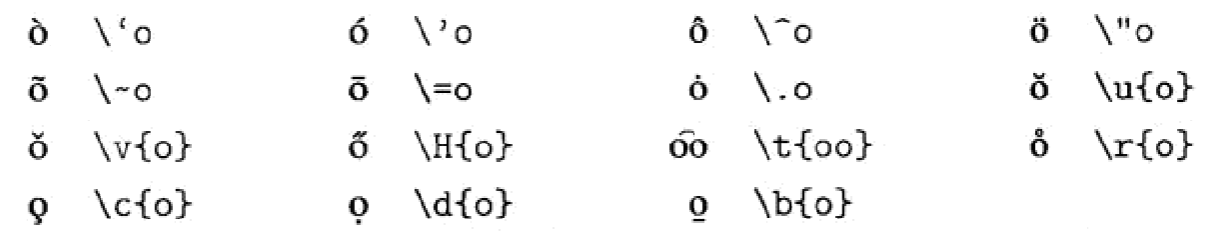
\includegraphics[width=9cm]{figures/zhongyin.png}
                    \caption{\LaTeX\ 中的重音符号, 以 $o$ 为例}
                    \label{fig:zhongyin}
                \end{figure}
                \begin{figure}[ht]
                    \centering
                    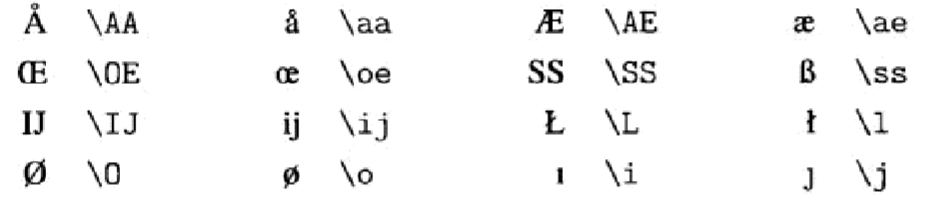
\includegraphics[width=9cm]{figures/teshu.PNG}
                    \caption{\LaTeX\ 中的特殊字母}
                    \label{fig:teshu}
                \end{figure}
                \begin{figure}[ht]
                    \centering
                    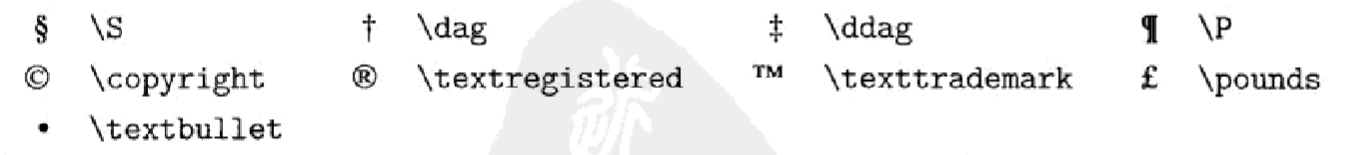
\includegraphics[width=9cm]{figures/teshufuhao.PNG}
                    \caption{\LaTeX\ 中的特殊符号}
                    \label{fig:teshufuhao}
                \end{figure}

                \item 字符输出连写. 
                \begin{itemize}
                    \item 通过空分组 \{\} 或 \textbackslash/ 取消
                    \item 或使用宏包选项
                \end{itemize}

            \end{enumerate}

        \subsubsection{标点符号}

            \begin{enumerate}

                \item 可直接使用的标点: 
                \\,\quad.\quad;\quad:\quad!\quad?\quad`\quad'\quad(\quad)\quad[\quad]\quad-\quad/\quad*\quad @

                \item 双引号以两个单引号合并, 以 \textbackslash , 分隔. 

                \item 符号 - 有多种用途: 
                \begin{itemize}
                    \item 数学模式中作减号
                    \item 单独使用时作连字符
                    \item 两个连用作 en dash 表示数字范围
                    \item 三个连用作 em dash 表示破折号
                \end{itemize}

                \item 省略号: 
                \begin{itemize}
                    \item 命令有: \textbackslash ldots, \textbackslash dots, \textbackslash ddot ( 数学模式中用 )
                    \item 后面会增加一个小间距 ( 同于中间间隔 )
                    \item 句中前后加空格 ( 应放入数学模式中, 以避免后间距过大 ) , 句末用四个点. 
                \end{itemize}

                \item 有些有特殊意义标点不能直接输入, 如: 
                \\\#\quad\$\quad\%\quad\&\quad\{\quad\}\quad\_\quad\textbackslash 它们通过在前面加 \textbackslash 得到. 
                \\ 又如 \~{} 和 \^{} 通过空组加重音显示. 
                \\ 像符号: $|\quad <\quad >\quad +\quad =$ 一般用于数学公式中, 其文本形式或出错 ( 前三个符号文本形式为: |\quad<\quad> ) 或效果不好. 

                \item 中文标点
                \begin{itemize}
                    \item 中文标点为全角
                    \item 一般直接以输入法输入
                    \item 科技文章中以全角 ``.''而非一般``.''
                \end{itemize}

            \end{enumerate}

        \subsubsection{空字符}

            \begin{enumerate}

                \item 空格与换行
                \begin{itemize}
                    \item 空格起分隔单词作用, 多空格作用同单个空格等效. 
                    \item 以字母命名的宏, 其后空格会被忽略. 
                    \item 空分组 \{\} 与 \textbackslash 空格 亦可作空格 ( 且后者不可被省去 )
                    \item 汉字与其他内容间自动产生空格 ( 可放入盒子取消其影响---\textbackslash \{\} )
                    \item $\sim$ ---带子, 可作为不可打断的空格, 连接作用. 
                \end{itemize}

                \item 换行
                \begin{itemize}
                    \item \LaTeX\ 根据页面宽度和字宽顿号间距及字数, 将空格转为换行符. 
                    \item 可用 \textbackslash\textbackslash 另起一行. ( 行文不常用 )
                    \item 或 \textbackslash linebreak --- 指定断点, 所断上部分按一行散开对齐. ( 行文不常用 )
                    \item 标点后空格作为换行是必须的 ( 换行用 )
                    \begin{itemize}
                        \item 句号前小写字母, 后空格间距比单词间空格 ( 普通 ) 大 ( 视为句子结尾 ) --- 用 \textbackslash 空格代替. 
                        \item 句号前大写, 间距普通 ( 视为缩写 ) --- 句号前加 \textbackslash @取消影响. 
                    \end{itemize}
                \end{itemize}

                \item 幻影
                \begin{itemize}
                    \item \textbackslash phantom\{\} 产生同参数内容长空盒子.
                    \item 类似有 \textbackslash hphantom ( 水平 ) 和 \textbackslash vphantom ( 垂直 ). 
                \end{itemize}

            \end{enumerate}

    \subsection{段落与文本环境}

            \subsubsection{分段}

                段与段直接, 垂直模式装并. 

                方式有: 
                \begin{itemize}
                    \item 空行
                    \item 用命令 \textbackslash par ( 主要用于命令或环境定义的内部 )
                \end{itemize}

                \textbackslash\textbackslash 不分段, 另起一行 ( 可加可选参数表示格外垂直间距 ). \textbackslash linebreak 指定一行断点, 上一行按完整一行散开对齐. 

    \subsection{文档层次结构}

        \LaTeX\ 结构化文本编写手段、方法.

        \subsubsection{标题与标题页}

            \begin{enumerate}

                \item 声明标题结构与内容. 如: 
                \begin{itemize}
                    \item 标题---\textbackslash title
                    \item 作者---\textbackslash author
                    \begin{itemize}
                        \item 参数可用 \textbackslash\textbackslash\ 分行
                        \item 多个作者参数则用 \textbackslash and 分隔
                        \item 可以使用 \textbackslash thanks 添加特殊脚注, 作为文章致谢、文档版本以及作者详细信息. 
                    \end{itemize}
                    \item 日期---\textbackslash date
                    \begin{itemize}
                        \item 省略 \textbackslash date 同于 \textbackslash date\{\textbackslash today\}
                        \item 可使用宏包 CTEXoptions 来另外设置 \textbackslash today 的输出格式
                    \end{itemize}
                \end{itemize}

                \item 实际输出标题
                \begin{itemize}
                    \item 使用 \textbackslash maketitle 输出已声明标题.
                    \item 输出随文档类而不同
                    \begin{description}
                        \item[article 和 ctexart] 标题不单独成页
                        \item[report, book 或 ctexrep, ctexbook] 单独占一页 
                        \item[此外] 可添加文档类的选项 titlepage 或 notitlepage 来设置成页与否
                    \end{description}
                \end{itemize}

                \item 直接手工排版标题页
                \begin{itemize}
                    \item 建立 titlepage 环境---不计入页码.\\
                        命令: 
                    \begin{description}
                        \item[居中] 环境 center
                        \item[标题外空间] 命令 vspace
                        \item[标题间空间分隔] 命令 bigskip, medskip
                        \item[字体命令] 大写, 样式   
                    \end{description}
                    \item 另外使用宏包 titling 详细设置. 
                \end{itemize}

            \end{enumerate}

\end{document}